\begin{tabular}{M{7cm}M{10.5cm}}
	\textbf{LỚP CÔ THẢO - THẦY SANG}& \textbf{ĐỀ ÔN TẬP KIỂM TRA CUỐI HỌC KÌ 1}\\
	\textbf{MÃ ĐỀ: 004}& \textbf{Bài thi môn: VẬT LÝ 12}\\
	\textit{(Đề trường THCS-THPT Lê Thánh Tông năm học 2024 - 2025)}& \textit{Thời gian làm bài: 50 phút, không kể thời gian phát đề}
	
	\noindent\rule{4cm}{0.8pt} \\
\end{tabular}
\setcounter{section}{0}
\section{Câu trắc nghiệm nhiều phương án lựa chọn}
\textit{Thí sinh trả lời từ câu 1 đến câu 18. Mỗi câu hỏi thí sinh chọn một phương án}
\setcounter{ex}{0}
\Opensolutionfile{ans}[ans/FINAL-SEM1-004-TN]
% ===================================================================
\begin{ex}
	Trong các đơn vị cho dưới đây, đơn vị nào không phải là đơn vị đo độ lớn cảm ứng từ?
	\choice
	{tesla $\left(\si{\tesla}\right)$}
	{\si{\newton\cdot\meter^{-1}\cdot\ampere^{-1}}}
	{\si{\kilogram\cdot\ampere^{-1}\cdot\second^{-1}}}
	{\True \si{\kilogram\cdot\ampere^{-1}\cdot\meter^{-2}}}
	\loigiai{}
\end{ex}
% ===================================================================
\begin{ex}
	Giả sử một nhiệt kế thủy ngân bị mất thông số vạch chia độ. Ở áp suất tiêu chuẩn, để xác định lại vị trí vạch $\SI{0}{\celsius}$ trên nhiệt kế thì cần đặt nhiệt kế vào đối tượng nào dưới đây?
	\choice
	{Ngăn đông của tủ lạnh}
	{Ngọn lửa của bếp ga}
	{\True Nước đá đang tan chảy}
	{Nước sôi}
	\loigiai{}
\end{ex}
% ===================================================================
\begin{ex}
	Chỉ ra phát biểu đúng khi nói về kim la bàn.
	\choice
	{Lực làm kim la bàn quay là lực hấp dẫn}
	{\True Bình thường, cực Bắc của kim la bàn chỉ về hướng Bắc địa lí}
	{Kim la bàn luôn luôn định hướng theo một phương xác định}
	{Kim la bàn chỉ chịu ảnh hưởng bởi từ trường của Trái Đất}
	\loigiai{}
\end{ex}
% ===================================================================
\begin{ex}
	Khi tăng khối lượng của chất rắn 3 lần thì nhiệt lượng cung cấp cho vật rắn nóng chảy hoàn toàn sẽ
	\choice
	{\True tăng lên 3 lần}
	{giảm đi 3 lần}
	{giảm đi 9 lần}
	{tăng lên 9 lần}
	\loigiai{}
\end{ex}
\textit{Sử dụng thông tin sau cho Câu 5 và Câu 6: Một đoạn dây dẫn thẳng mang dòng điện có cường độ $\SI{6}{\ampere}$ ở trong từ trường đều có độ lớn cảm ứng từ là $\SI{4}{\milli\tesla}$, biết góc hợp bởi vectơ cảm ứng từ với đoạn dây dẫn có dòng điện là $\alpha$.}
% ===================================================================
\begin{ex}
	Khi $\alpha=\SI{30}{\degree}$ thì lực từ tác dụng lên một đơn vị chiều dài là
	\choice
	{\True \SI{0.012}{\newton/\meter}}
	{\SI{12}{\newton/\meter}}
	{\SI{0.021}{\newton/\meter}}
	{\SI{0.024}{\newton/\meter}}
	\loigiai{$\dfrac{F}{\ell}=IB\sin\alpha=\SI{0.012}{\newton/\meter}$.}
\end{ex}
% ===================================================================
\begin{ex}
	Nếu thay đổi góc $\alpha$ thì lực từ tác dụng lên đoạn dây có độ lớn lớn nhất khi
	\choice
	{\True $\alpha=\SI{90}{\degree}$}
	{$\alpha=\SI{0}{\degree}$}
	{$\alpha=\SI{30}{\degree}$}
	{$\alpha=\SI{45}{\degree}$}
	\loigiai{}
\end{ex}
% ===================================================================
\begin{ex}
	\immini{Tàu đệm từ là một phương tiện giao thông chạy trên đệm từ trường, tàu vận hành rất êm, không rung lắc và không gây ra nhiều tiếng ồn như tàu truyền thống. Tàu sử dụng cơ chế nâng, đẩy và dẫn lái để khi di chuyển với tốc độ cao mà tàu không bay khỏi bề mặt đường ray. Trong hình vẽ bên mô tả cơ chế nâng để nâng tàu lên trong quá trình tàu di chuyển. Các cực từ ở các vị trí (1), (2) và (3) theo đúng thứ tự là}
	{\vspace{-0.5cm}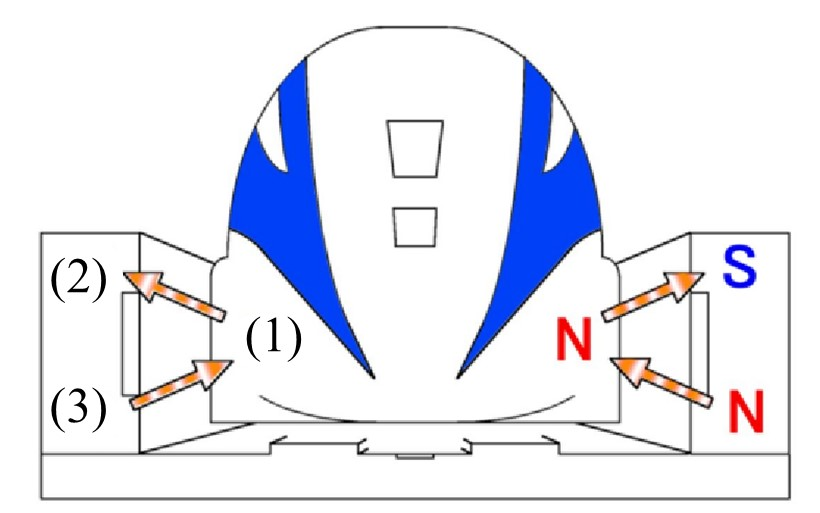
\includegraphics[scale=0.4]{../figs/FINAL-SEM1-004-1}}
	\choice
	{\True S-N-S}
	{N-N-N}
	{S-S-N}
	{N-N-S}
	\loigiai{}
\end{ex}
% ===================================================================
\begin{ex}
Nội dung nào dưới đây \textbf{không phải} là tính chất của các phân tử khí?	
	\choice
	{Chuyển động hỗn loạn, không ngừng}
	{Nhiệt độ càng cao, các phân tử khí chuyển động càng nhanh}
	{Các phân tử khí va chạm vào thành bình gây ra áp suất}
	{\True Chuyển động hỗn loạn xung quanh các vị trí cân bằng cố định}
	\loigiai{}
\end{ex}
% ===================================================================
\begin{ex}
	Khi một lượng khí lí tưởng xác định dãn nở đẳng nhiệt thì mật độ phân tử khí sẽ
	\choice
	{tăng tỉ lệ nghịch với áp suất}
	{\True giảm tỉ lệ thuận với áp suất}
	{không thay đổi}
	{tăng tỉ lệ thuận với áp suất}
	\loigiai{}
\end{ex}
% ===================================================================
\begin{ex}
	Một khối khí helium có động năng tịnh tiến trung bình của mỗi phân tử là $\SI{0.1}{\electronvolt}$. Nhiệt độ của khối khí khi đó là
	\choice
	{$\SI{500}{\kelvin}$}
	{\True $\SI{773}{\kelvin}$}
	{$\SI{483}{\kelvin}$}
	{$\SI{128.4}{\kelvin}$}
	\loigiai{
	$W_{\text{đ}}=\dfrac{3}{2}kT\Leftrightarrow 0,1\cdot1,6\cdot10^{-19}=\dfrac{3}{2}\cdot1,38\cdot10^{-23}T\Rightarrow T\approx\SI{773}{\kelvin}$.
	}
\end{ex}
% ===================================================================
\begin{ex}
	\immini{Cho sơ đồ mạch điện và kim nam châm được treo như hình vẽ bên. Khi đóng công tắc K thì kim nam châm sẽ
		\choice
		{bị hút sang trái}
		{\True bị đẩy sang phải}
		{vẫn đứng yên}
		{bị hút sang trái rồi đẩy sang phải}}
		{\vspace{-0.5cm}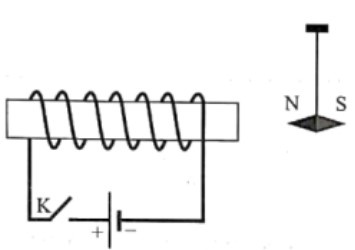
\includegraphics[scale=0.6]{../figs/FINAL-SEM1-004-2}}
	\loigiai{}
\end{ex}
% ===================================================================
\begin{ex}
	Tăng đồng thời nhiệt độ và áp suất của một khối khí lí tưởng từ $\SI{27}{\celsius}$ lên $\SI{177}{\celsius}$ và từ $\SI{100}{\kilo\pascal}$ lên $\SI{300}{\kilo\pascal}$. Khối lượng riêng của khối khí tăng hay giảm bao nhiêu lần?
	\choice
	{Giảm 2 lần}
	{Giảm 3 lần}
	{\True Tăng 2 lần}
	{Tăng 3 lần}
	\loigiai{
	$\dfrac{p}{DT}=const\Rightarrow \dfrac{100\cdot10^3}{D_1\cdot\left(27+273\right)}=\dfrac{300\cdot10^3}{D_2\cdot\left(177+273\right)}\Rightarrow \dfrac{D_2}{D_1}=2$.
	}
\end{ex}
\textit{Sử dụng thông tin sau cho Câu 13 và Câu 14: Một đoạn dây thẳng bằng đồng được đặt vuông góc với một từ trường đều. Trong đoạn dây có dòng điện với cường độ $\SI{6}{\ampere}$ và có phương chiều như hình vẽ. Bỏ qua ảnh hưởng từ trường Trái Đất lên đoạn dây. Biết khối lượng của một đơn vị chiều dài của đoạn dây đồng là $\SI{46.6E-3}{\kilogram/\meter}$; lấy $g=\SI{9.8}{\meter/\second^2}$. Để lực từ cân bằng với lực hút của Trái Đất tác dụng lên đoạn dây thì:}
% ===================================================================
\begin{ex}
	\immini{Phương và chiều của cảm ứng từ là
		\choice
		{phương nằm ngang và chiều từ trái qua phải}
		{\True phương nằm ngang và chiều từ phải qua trái}
		{phương thẳng đứng và chiều từ dưới lên trên}
		{phương thẳng đứng và chiều trên xuống dưới}}
	{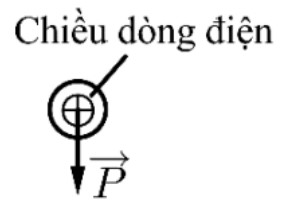
\includegraphics[scale=0.6]{../figs/FINAL-SEM1-004-3}}
	\loigiai{}
\end{ex}
% ===================================================================
\begin{ex}
	Độ lớn tối thiểu của cảm ứng từ là
	\choice
	{$\SI{0.76}{\tesla}$}
	{\True $\SI{0.076}{\tesla}$}
	{$\SI{0.29}{\tesla}$}
	{$\SI{0.029}{\tesla}$}
	\loigiai{
	$F=P\Rightarrow I\ell B=mg\Rightarrow B=\dfrac{mg}{I\ell}\approx\SI{0.076}{\tesla}$.
	}
\end{ex}
% ===================================================================
\begin{ex}
	Một khối khí lí tưởng xác định thực hiện quá trình biến đổi đẳng nhiệt ở hai nhiệt độ khác nhau $T_1$ và $T_2$ (trong đó $T_2<T_1$ ). Hình nào dưới đây diễn tả đúng dạng đường đẳng nhiệt trong hệ tọa độ tương ứng?
	\begin{center}
		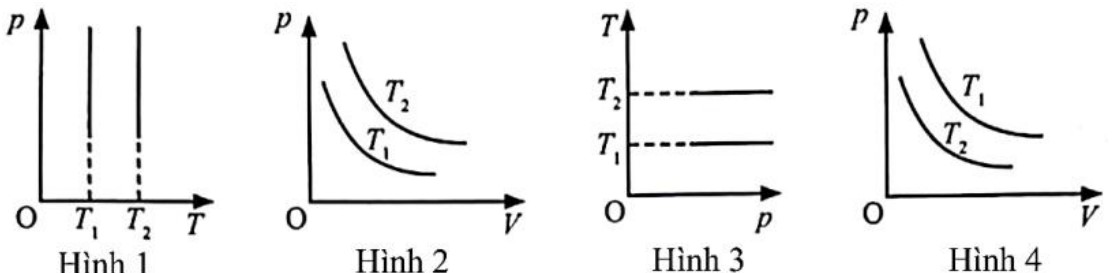
\includegraphics[scale=0.7]{../figs/FINAL-SEM1-004-4}
	\end{center}
	\choice
	{Hình 1}
	{Hình 2}
	{Hình 3}
	{\True Hình 4}
	\loigiai{}
\end{ex}
% ===================================================================
\begin{ex}
	\immini{Một khối khí lý tưởng xác định có khối lượng không đổi, biến đổi từ trạng thái I đến trạng thái II, thể tích thay đổi theo nhiệt độ như đồ thị ở hình vẽ. Trong quá trình này áp suất khí
		\choice
		{\True Tăng}
		{Giảm}
		{Không đổi}
		{Tăng rồi giảm}}
		{\vspace{-0.5cm}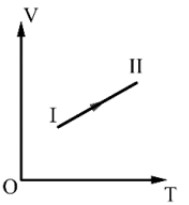
\includegraphics[scale=0.8]{../figs/FINAL-SEM1-004-5}}
	\loigiai{
	$V=aT+V_0$ mà $V=\dfrac{nRT}{p}\Rightarrow p=\dfrac{nR}{a+\dfrac{V_0}{T}}$.\\
	Trong quá trình (I) $\rightarrow$ (II) thì $T$ tăng nên $p$ tăng.
	}
\end{ex}
\textit{Sử dụng thông tin sau cho Câu 17 và Câu 18: Xét một đoạn dây dẫn dài 50 cm đặt trong từ trường đều có độ lớn cảm ứng từ \SI{4}{\milli\tesla}, theo phương vuông góc với đường sức từ. Biết rằng trong mỗi giây có \SI{2E18}{electron} đi qua một tiết diện thẳng trong dây dẫn.}
% ===================================================================
\begin{ex}
	Cường độ dòng điện chạy qua dây dẫn bằng bao nhiêu?
	\choice
	{\True \SI{0.32}{\ampere}}
	{\SI{3.2}{\ampere}}
	{\SI{1.6}{\ampere}}
	{\SI{0.16}{\ampere}}
	\loigiai{
	$i=\dfrac{q}{t}=\dfrac{ne}{t}=\SI{0.32}{\ampere}$.
	}
\end{ex}
% ===================================================================
\begin{ex}
	Độ lớn lực từ tác dụng tác dụng lên dây dẫn là
	\choice
	{\True \SI{6.4E-4}{\newton}}
	{\SI{64E-4}{\newton}}
	{\SI{32E-4}{\newton}}
	{\SI{3.2E-4}{\newton}}
	\loigiai{
	$F=I\ell B=0,32\cdot0,5\cdot4\cdot10^{-3}=\SI{6.4E-4}{\newton}$.
	}
\end{ex}
\Closesolutionfile{ans}
\section{Câu trắc nghiệm đúng/sai} 
\textit{Thí sinh trả lời từ câu 1 đến câu 4. Trong mỗi ý \textbf{a)}, \textbf{b)}, \textbf{c)}, \textbf{d)} ở mỗi câu, thí sinh chọn đúng hoặc sai}
\setcounter{ex}{0}
\Opensolutionfile{ans}[ans/FINAL-SEM1-004-TF]
% ===================================================================
\begin{ex}
	\immini{Bóng đèn sợi đốt (bóng đèn dây tóc) còn được gọi tắt là bóng đèn tròn (Hình vẽ), là loại bóng đèn trước đây được sử dụng rộng rãi trong cuộc sống. Trong lĩnh vực nông nghiệp, đèn sợi đốt được người dân sử dụng để kích thích cây ra hoa trái vụ, thu hoạch được sản lượng cao hơn. Bộ phận chính của đèn sợi đốt gồm: sợi đốt làm bằng wolfram, chịu được nhiệt độ cao; bóng thuỷ tinh làm bằng thuỷ tinh chịu nhiệt, bên trong được bơm khí trơ ở áp suất thấp.}
	{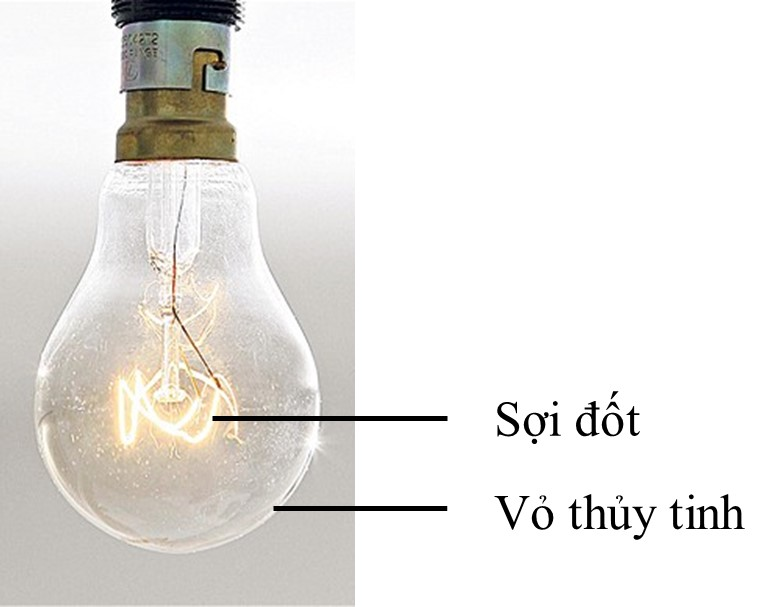
\includegraphics[scale=0.3]{../figs/FINAL-SEM1-004-6}}
	\choiceTF[t]
	{Khi bóng đèn hoạt động thì điện năng biến đổi trực tiếp thành quang năng}
	{\True Sợi đốt làm bằng kim loại wolfram vì có nhiệt độ nóng chảy cao}
	{\True Sử dụng khí trơ ở áp suất thấp để làm giảm oxi hóa sợi đốt khi chiếu sáng}
	{\True Bóng đèn sợi đốt có lớp vỏ làm bằng thuỷ tinh chịu nhiệt nên nhiệt độ khi đèn sáng có thể đạt tới $\SI{260}{\celsius}$, coi áp suất khí trong bóng đèn bằng với áp suất khí quyển là $\SI{1}{atm}$. Áp suất khí trong bóng đèn khi đèn chưa sáng ở nhiệt độ $\SI{26}{\celsius}$ là $\SI{0.56}{atm}$. Bỏ qua mọi sự trao đổi nhiệt với môi trường.}
	\loigiai{}
\end{ex}
% ===================================================================
\begin{ex}
	Một nhóm học sinh thực hành đo nhiệt dung riêng của nước.
	\begin{center}
		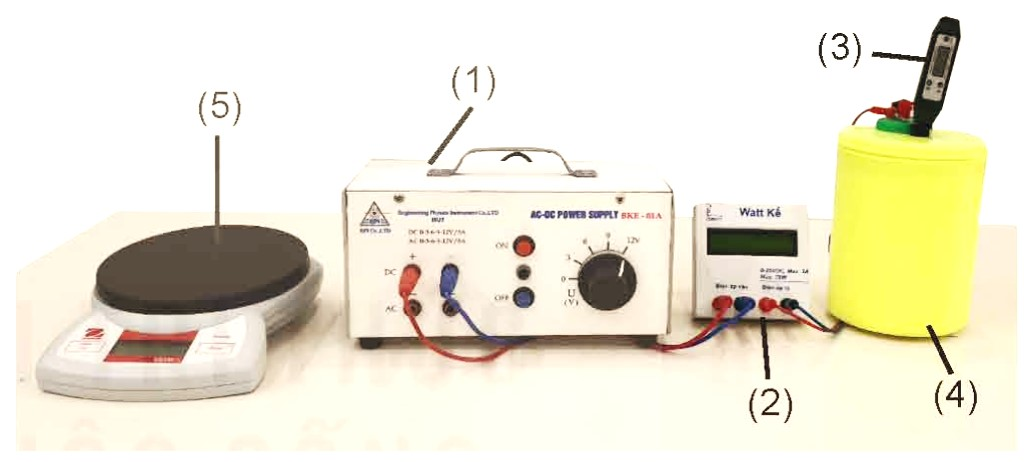
\includegraphics[scale=0.35]{../figs/FINAL-SEM1-004-7}
	\end{center}
	\begin{center}
		\begin{tabular}{|M{7cm}|M{10cm}|}
			\hline
			\textbf{Dụng cụ thí nghiệm gồm:} & \textbf{Các bước tiến hành thí nghiệm:}\\
			\begin{itemize}[-]
				\item Biến thế nguồn (1).
				\item Bộ đo công suất nguồn điện (oát kế) có tích hợp chức năng đo thời gian (2).
				\item Nhiệt kế điện tử (3).
				\item Nhiệt lượng kế bằng nhựa có vỏ xốp, kèm dây điện trở (gắn ở mặt trong của nắp bình) (4).
				\item Cân điện tử (5).
				\item Các dây nối.
			\end{itemize}
			&
			\begin{enumerate}[label=\alph*)]
				\item Cắm đầu đo của nhiệt kế vào nhiệt lượng kế.
				\item Bật nguồn điện.
				\item Nối oát kế với nhiệt lượng kế và nguồn điện.
				\item Đổ một lượng nước vào bình nhiệt lượng kế, sao cho toàn bộ dây điện trở chìm trong nước, xác định khối lượng nước này. 
				\item Khuấy liên tục để nước nóng đều. Cứ sau mỗi khoảng thời gian 3 phút, đọc công suất dòng điện từ oát kế, nhiệt độ từ nhiệt kế rồi ghi lại kết quả.
				\item Tắt nguồn điện.
			\end{enumerate}\\
			\hline
		\end{tabular}
	\end{center}
	\begin{center}
		\begin{tabular}{|M{2cm}|M{4.5cm}|M{4.5cm}|M{4.5cm}|}
			\hline
			\multicolumn{4}{|M{15.5cm}|}{Khối lượng nước $m=\SI{0.136}{\kilogram}$; Nhiệt độ ban đầu: $\SI{27}{\celsius}$}\\
			\hline
			Lần đo & Thời gian đun $\xsi{\Delta t}{\left(\second\right)}$ & Nhiệt độ nước sau đun $\left(\si{\celsius}\right)$ & Công suất đun $\xsi{\calP}{\left(\watt\right)}$\\
			\hline
			1 & 180 & 33 & 18,2\\
			\hline
			\dots &&&\\
			\hline
		\end{tabular}
	\end{center}
	\choiceTF[t]
	{\True Thứ tự đúng các bước tiến hành thí nghiệm là: d, a, c, b, e, f}
	{\True Nhiệt lượng mà nước thu vào bằng điện năng đã cung cấp cho dây điện trở trong nhiệt lượng kế}
	{\True Với kết quả thí nghiệm trong lần đo 1, nhóm học sinh xác định được nhiệt dung riêng của nước là \SI{4014.71}{\joule/\kilogram\cdot\kelvin}}
	{\True Để có kết quả gần giá trị thực tế hơn thì nhóm học sinh cần lặp lại thí nghiệm nhiều lần rồi lấy giá trị trung bình}
	\loigiai{
	\begin{itemchoice}
		\itemch Đúng.
		\itemch Đúng.
		\itemch Đúng. $\calP\Delta t=mg\left(t-t_0\right)\Rightarrow 18,2\cdot180=0,136c\cdot\left(33-27\right)\Rightarrow c\approx\SI{4014.71}{\joule/\kilogram\cdot\kelvin}$.
		\itemch Đúng.
	\end{itemchoice}
	}
\end{ex}
% ===================================================================
\begin{ex}
	\immini{Hình vẽ bên là sơ đồ nguyên lý của một khẩu súng phun nước. Khi bóp hết cò súng thì áp suất do pít tông gây ra được nước truyền nguyên vẹn tới vòi phun. Biết: tiết diện của pít tông và vòi phun tương ứng là $\SI{2.1}{\centi\meter^2}$ và $\SI{0.09}{\centi\meter^2}$; khối lượng riêng của nước là $\SI{1.0}{\gram/\centi\meter^3}$, lượng nước phun ra mỗi lần bóp cò là như nhau. Khi tác dụng lực có độ lớn $\SI{4.2}{\newton}$ vào cò súng làm pít tông dịch chuyển $\SI{2.2}{\centi\meter}$.}
	{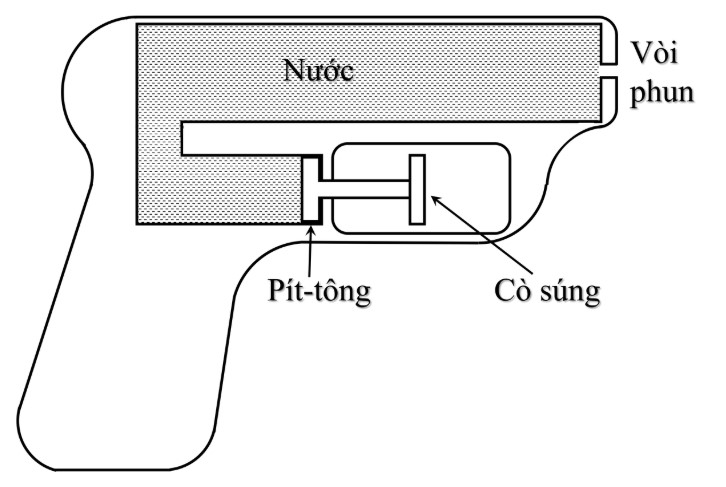
\includegraphics[scale=0.4]{../figs/FINAL-SEM1-004-8}}
	\choiceTF[t]
	{\True Áp suất do pít - tông gây ra bằng áp suất ở vòi phun}
	{\True Áp lực mà nước tạo ra tại vòi phun là $\SI{0.18}{\newton}$}
	{\True Mỗi lần bóp cò thì khối lượng nước phun ra ở vòi phun là $\SI{4.62}{\gram}$}
	{Công thực hiện cho mỗi lần bóp cò là $\SI{3.96E-3}{\joule}$}
	\loigiai{\begin{itemchoice}
			\itemch Đúng. Theo nguyên lý Pascal, áp suất được truyền nguyên vẹn tới mọi điểm trong lòng chất lỏng.\\
			\itemch Đúng. $p=\dfrac{F_{pt}}{S_{pt}}=\dfrac{F_{vp}}{S_{vp}}\Rightarrow \dfrac{4,2}{2,1}=\dfrac{F_{vp}}{0,09}\Rightarrow F_{vp}=\SI{0.18}{\newton}$.
			\itemch Đúng. $\Delta V=S_{pt}\cdot S=\SI{4.62}{\centi\meter^3}$; $\Delta m=D\Delta V=\SI{4.62}{\gram}$.
			\itemch Sai. $A=F_{pt}S=\SI{0.0924}{\joule}$.
	\end{itemchoice}}
\end{ex}
% ===================================================================
\begin{ex}
	\immini{Cho hai dây dẫn thẳng song song, dài vô hạn lần lượt có dòng điện $I_1$ và $I_2$ chạy qua như hình vẽ bên. Xét mặt phẳng $\left(Oxy\right)$ vuông góc với cả hai dòng điện, cắt các dòng điện tại A và B với $\mathrm{AB}=\SI{12}{\centi\meter}$.}
	{\vspace{-0.5cm}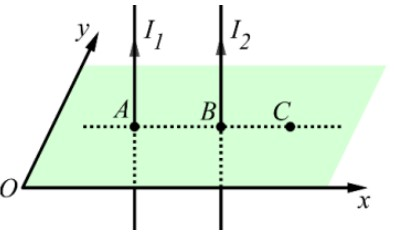
\includegraphics[scale=0.6]{../figs/FINAL-SEM1-004-9}}
	\choiceTF[t]
	{\True Hai dòng điện $I_1$ và $I_2$ hút nhau}
	{\True Các vectơ cảm ứng từ do hai dòng điện $I_1$ và $I_2$ gây ra tại điểm C (A, B, C thẳng hàng) cùng chiều nhau và cùng chiều với trục $Oy$}
	{\True Nếu đặt kim la bàn tại điểm C thì kim la bàn sẽ chỉ hướng từ Nam đến Bắc cùng chiều với trục $Oy$}
	{\True Nếu $I_1=I_2=\SI{10}{\ampere}$. Điểm M thuộc mặt phẳng $\left(Oxy\right)$ và cách đều hai dòng điện $I_1$ và $I_2$ một khoảng $x$. Để độ lớn cảm ứng từ tổng hợp tại điểm $M$ đạt giá trị lớn nhất thì $x \approx \SI{8.5}{\centi\meter}$}
	\loigiai{\immini{\begin{itemchoice}
				\itemch Đúng. Hai dòng điện $I_1$ và $I_2$ cùng chiều nên hút nhau.
				\itemch Đúng. Áp dụng quy tắc nắm tay phải, xác định được vector cảm ứng từ do hai dòng điện $I_1$ và $I_2$ gây ra tại điểm C (A, B, C thẳng hàng) cùng chiều nhau và cùng chiều với trục $Oy$.
				\itemch Đúng.
				\itemch Đúng. $B_1=B_2=2\cdot10^{-7}\cdot\dfrac{I}{x}$.\\
				$B=2B_1\cos\alpha=2\cdot\SI{2E-7}{}\cdot\dfrac{I}{x}\cdot\dfrac{h}{x}=\dfrac{\SI{4E-7}{}Ih}{h^2+a^2}=\dfrac{\SI{4E-7}{}I}{h+\dfrac{a^2}{h}}$.\\
				Áp dụng bất đẳng thức Cauchy:
				$$B\le\dfrac{\SI{4E-7}{}I}{2a}.$$
				Dấu "=" xảy ra khi $h=\dfrac{a^2}{h}\Rightarrow h=a\Rightarrow x=a\sqrt{2}\approx\SI{8.5}{\centi\meter}$.
	\end{itemchoice}}
{\vspace{3cm}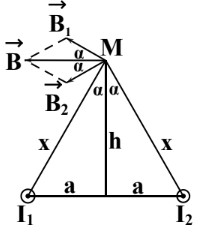
\includegraphics[scale=0.8]{../figs/FINAL-SEM1-004-12}}
}
\end{ex}
\Closesolutionfile{ans}
\section{Câu trắc nghiệm trả lời ngắn} \textit{Thí sinh trả lời từ câu 1 đến câu 6}
\setcounter{ex}{0}
\Opensolutionfile{ans}[ans/FINAL-SEM1-004-TL]
% ===============================================================
\begin{ex}
	Một bình chứa oxygen xem là khí lý tưởng sử dụng trong y tế có thể tích 14 lít, áp suất $\SI{15E6}{\pascal}$ và nhiệt độ phòng $\SI{27}{\celsius}$. Biết khối lượng mol của oxygen là $\SI{32}{\gram/\mole}$. Khối lượng oxygen trong bình bằng bao nhiêu kilogam (làm tròn kết quả đến chữ số hàng phần mười)?
	\shortans[oly]{2,7}
	\loigiai{
		$pV=\dfrac{m}{M}RT\Rightarrow m=\SI{2.7}{\kilogram}$.
	}
\end{ex}
% ===============================================================
\begin{ex}
	\immini{Một quyển sách khoa học cổ được phát hiện tại một hòn đảo thuộc Ấn Độ Dương vào thế kỷ 18 . Trong cuốn sách này có một bài toán nhỏ dịch sang Tiếng Việt như sau: "Một pinch khí được chứa trong một bình kín có thể tích 1,5 volka. Khi nhiệt độ là 40 tapu thì áp suất khí là 25 phatka. Khi nhiệt độ giảm xuống tới $-20$ tapu thì áp suất khí là 10 phatka". Nếu ta giả sử chất khí mà bài toán đó đang đặt ra là khí lý tưởng và tuân theo các định luật của khí lý tưởng. Độ không tuyệt đối theo tapu là bao nhiêu (làm tròn kết quả đến chữ số hàng đơn vị)?}
	{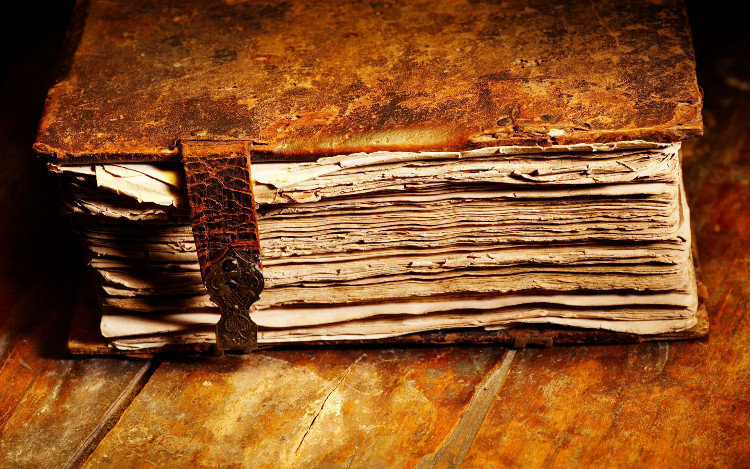
\includegraphics[scale=0.15]{../figs/FINAL-SEM1-004-10}}
	\shortans[oly]{ $-60$}
	\loigiai{
		Đẳng tích $p=cT=at+b\Rightarrow\begin{cases}
			25=40a+b\\
			10=-20a+b
		\end{cases}\Rightarrow\begin{cases}
		a=0,25\\
		b=15
		\end{cases}$.\\
		Độ không tuyệt đối là $T=0\Rightarrow 0,25t+15=0\Rightarrow t=-60$.
	}
\end{ex}
% ===============================================================
\begin{ex}
Đặt \SI{1.0}{\kilogram} nước ở \SI{25}{\celsius} vào tủ lạnh thì sau 65 phút, lượng nước này chuyển thành băng (nước đá) ở \SI{-14.5}{\celsius}. Cho biết nhiệt nóng chảy riêng và nhiệt dung riêng của băng lần lượt là \SI{0.34}{\mega\joule/\kilogram} và \SI{2.1}{\kilo\joule/\kilogram}; nhiệt dung riêng của nước là \SI{4.2}{\kilo\joule/\kilogram\cdot\kelvin}. Công suất làm lạnh của tủ lạnh bằng bao nhiêu kilowatt $\left(\si{\kilo\watt}\right)$ (làm tròn kết quả đến chữ số hàng phần trăm)?	
	\shortans[oly]{0,12}
	\loigiai{
		$Q=m\left(c_n\Delta t_n+\lambda +c_b\Delta t_b\right)=\SI{475.45}{\kilo\joule}$.\\
		$\calP=\dfrac{Q}{t}=\dfrac{475,45}{65\cdot60}\approx\SI{0.12}{\kilo\watt}$.
	}
\end{ex}
% ===============================================================
\begin{ex}
	Một ống nghiệm tiết diện đều có chiều dài \SI{60}{\centi\meter}, đặt thẳng đứng chứa một khối khí đến \SI{40}{\centi\meter} ống, phần còn lại phía trên của ống là một cột thủy ngân. Nhiệt độ lúc đầu của khối khí là \SI{0}{\celsius}. Áp suất khí quyển là \SI{76}{\centi\meter Hg}. Để một nửa cột thủy ngân trào ra ngoài thì phải đun nóng khối khí lên đến bao nhiêu độ C (làm tròn kết quả đến chữ số hàng phần mười)?
	\shortans[oly]{ 32,7}
	\loigiai{
		Chiều cao cột thủy ngân ban đầu là $60-40=\SI{20}{\centi\meter}\Rightarrow$ lúc sau là $\dfrac{20}{2}=\SI{10}{\centi\meter}$.\\
		\begin{center}
			\begin{tabular}{|M{5cm}|M{5cm}|M{5cm}|}
				\hline
				$p$ & $V$ & $T$\\
				\hline
				$76+20=\SI{96}{\centi\meter Hg}$ & $\xsi{40\cdot S}{\centi\meter^3}$ & $\SI{273}{\kelvin}$\\
				\hline
				$76+10=\SI{86}{\centi\meter Hg}$ & $\xsi{\left(60-10\right)\cdot S}{\centi\meter^3}$ & $T_2$\\
				\hline
			\end{tabular}
		\end{center}
		$\dfrac{p_1V_1}{T_1}=\dfrac{p_2V_2}{T_2}\Rightarrow \dfrac{96\cdot S\cdot40}{273}=\dfrac{86\cdot S\cdot50}{T_2}\Rightarrow T_2\approx\SI{305.7}{\kelvin}\Rightarrow t\approx\SI{32.7}{\celsius}$.
	}
\end{ex}
\immini{\textit{Sử dụng các thông tin sau cho Câu 5 và Câu 6: Một thanh dẫn điện đồng chất có khối lượng $m=\SI{8}{\gram}$, dài $\ell=\SI{0.8}{\meter}$ được treo trong từ trường đều có phương vuông góc với mặt phẳng hình vẽ, chiều từ ngoài vào trong. Đầu trên O của thanh có thể quay tự do xung quanh một trục nằm ngang. Khi cho dòng điện cường độ $I=\SI{6}{\ampere}$ qua thanh thì khi cân bằng, đầu dưới M của thanh di chuyển một đoạn $d=\SI{2.1}{\centi\meter}$. Lấy $g=\SI{9.8}{\meter/\second^2}$.}}
{\vspace{-0.25cm}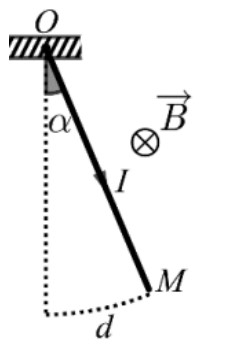
\includegraphics[scale=0.6]{../figs/FINAL-SEM1-004-11}}
% ===============================================================
\begin{ex}
	Cảm ứng từ $B$ có độ lớn là $\xsi{x \cdot 10^{-4}}{\tesla}$. Tìm giá trị của $x$ (làm tròn kết quả đến chữ số hàng phần mười).
	\shortans[oly]{4,3}
	\loigiai{
		$\sin\alpha=\dfrac{F}{P}\Rightarrow\sin\dfrac{d}{\ell}=\dfrac{I\ell B}{mg}\Leftrightarrow sin\dfrac{2,1\cdot10^{-2}}{0,8}=\dfrac{6\cdot0,8B}{8\cdot10^{-3}\cdot9,8}\Rightarrow B\approx\SI{4.3E-4}{\tesla}$.
	}
\end{ex}
% ===============================================================
\begin{ex}
	Đổi chiều dòng điện nhưng độ lớn vẫn không đổi. Sau khi thanh cân bằng thì điểm M dưới thanh đã di chuyển được một đoạn bằng bao nhiêu \si{\centi\meter} (làm tròn kết quả đến chữ số hàng phần mười)?
	\shortans[oly]{4,2 }
	\loigiai{
		Đổi chiều dòng điện thì lực từ đổi chiều nên vị trí cân bằng vẫn hợp với phương thẳng đứng góc $\alpha$ nhưng nằm ở bên trái $\Rightarrow$ thanh di chuyển đoạn $2d=2\cdot2,1=\SI{4.2}{\centi\meter}$.}
\end{ex}
\Closesolutionfile{ans}
\begin{center}
	\textbf{--- HẾT ---}
\end{center}
